\section{Hardware}

\subsection{VR Headset}\label{sec:vr-headset}

VR Headsets gibt es auf dem Markt schon viele.
Nach einer Statistik in 2017 sind die beliebtesten VR Headset Hersteller Sony, Oculus und HTC (Siehe~\ref{fig:vr_headset_manufacturer_marketshare}\cite{MARTINDALE_2017} gefunden in~\cite{CANKAYA_2019}).

\begin{figure}
    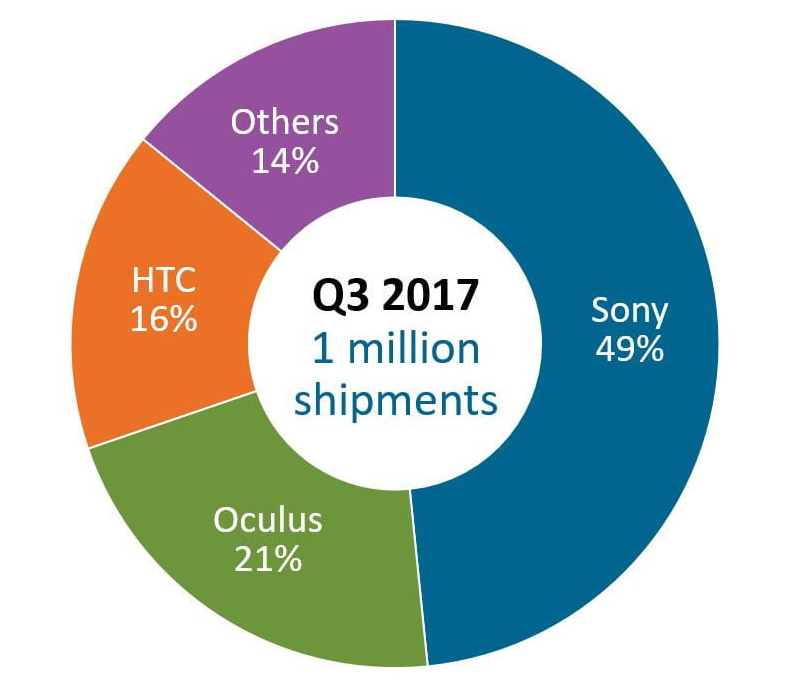
\includegraphics[scale=0.5]{pics/vr_headset_manufacturer_marketshare}
    \caption{Marketshare VR Headset Hersteller}
    \label{fig:vr_headset_manufacturer_marketshare}
\end{figure}

\subsubsection{HTC Vive Pro}

Die HTC Vive Pro

\subsection{VR Controller}\label{sec:vr-controller}

\subsection{Tracker}\label{sec:tracker}

\subsubsection{Vive Tracker}\label{sec:vive-tracker}

\subsection{Lichtboxen}\label{sec:lighthouse}

\subsection{Wireless Adapter }

\section{Software}

\subsection{Game Engine}

Es gibt mehrere Games Engines mit welchen eine VR Applikation geschrieben werden kann.
In Abbildung~\ref{fig:game_engine_marketshare} kann man den market share verschiedener Engines sehen.
Diese Daten sind aber mit vorsicht zu genießen, da das Skript welche diese Daten geliefert hat nach einigen Kriterien handelt.
Siehe~\cite{REDDIT_2018}.

\begin{figure}
    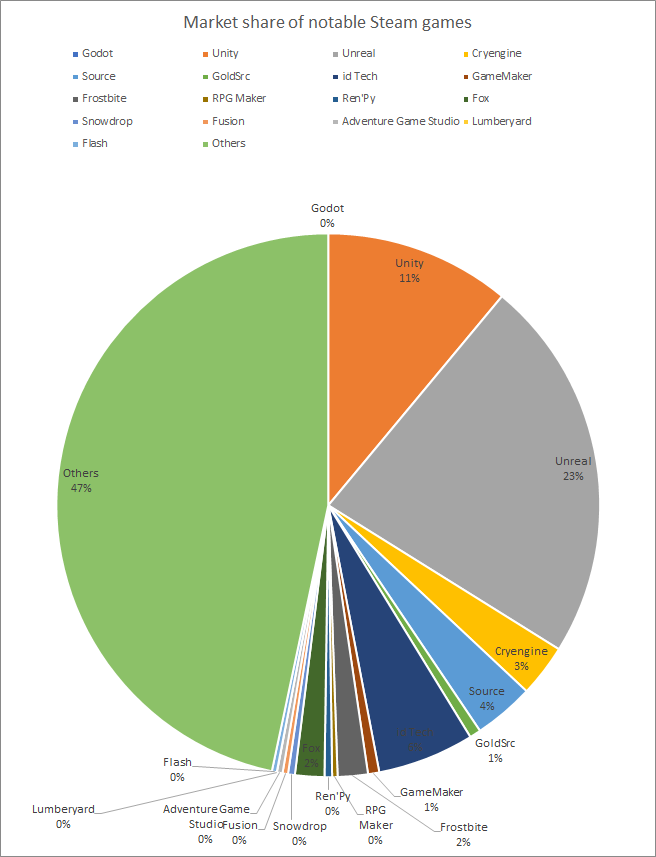
\includegraphics[scale=0.5]{pics/game_engine_marketshare}
    \caption{Game Engine Market-share}
    \label{fig:game_engine_marketshare}
\end{figure}

\begin{figure}
    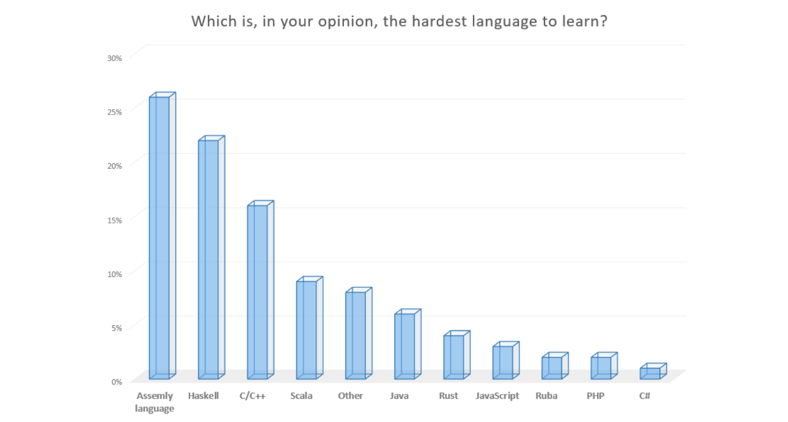
\includegraphics[scale=0.5]{pics/programming_languages_hardest}
    \caption{Schwerste Programmiersprachen}
    \label{fig:hardest_programming_languages}
\end{figure}

\subsubsection{Unity}

Unity ist eine Game Engine welche erstmals eine Apple exklusive Game Engine war und von Unity Technologies entwickelt worden ist.
Die Engine wurde weiter entwickelt und kann heute auch auf Windows und auf der Linux plattform benützt werden.
Die Engine ist gratis und wird von vielen als Einsteiger Engine beschrieben.
Auch sie eine Einsteiger Engine genannt wird heißt das nicht, dass sie in keinen professionellen Bereich benützt wird.
Viele bekannte Spiele wurden mit der Unity Engine entwickelt.
Im Besonderen sind viele Handyspiele mit dieser Engine entwickelt.
Spiele wie Pokemon GO, Among us und Hearthstone wurden in der Unity Engine entwickelt.

Vorteile:

\begin{itemize}
    \item Gratis Lizenz für persönlichen Nutzen und für Unternehmen mit unter 100000\$ Einkommen
    \item Programmierbar in der C\# Programmiersprache
    \item Es kann f\"ur alle moeglichen Plattformen ein Programm geschrieben werden
    \begin{itemize}
        \item IOS
        \item Android
        \item Windows
        \item Linux
        \item usw.
    \end{itemize}
    \item verfügbaren Asset-store mit vielen verschiedenen fertigen Assets
\end{itemize}

Nachteile:

\begin{itemize}
    \item weniger Market-share~\ref{fig:game_engine_marketshare}
    \item geschlossener Source Code
\end{itemize}

\subsubsection{Unreal Engine}
\label{sec:unreal_engine}

Unreal Engine ist von Epic Games entwickelt.
Diese Engine ist eine weit verwendete Game Engine.
Dies kann man auch in Abbildung~\ref{fig:game_engine_marketshare} herausnehmen.
Unreal Engine findet ihren nutzen aber eher in der PC- und Konsolen-welt.
Viele Spiele wie Fortnite, Ark Survival Evolved, Borderlands 3 und Jedi Fallen Order sind mit dieser Engine entwickelt worden.

Vorteile:

\begin{itemize}
    \item großer Market-share~\ref{fig:game_engine_marketshare}
    \item 'easy to learn' visual scripting
\end{itemize}

Nachteile

\begin{itemize}
    \item 5\% Nutzungshonorar, wenn das Einkommen eines Produktes über 1000000\$ ist
    \item für erweiterte funktionalität wird c++ welches nach Umfrage in der Abbildung~\ref{fig:hardest_programming_languages}~\cite{JAXCENTER_2018} die drittschwierigste Sprache ist
\end{itemize}

\subsubsection{Source Engine und Source 2 Engine}

Source Engine ist eine Game Engine welche von Steam/Valve entwickelt worden ist.
Diese Engine wurde im Jahre 2010 durch Source 2 ersetzt, welche verantwortlich ist für Spiele wie Dota 2 und Half Life Alyx.
Andere Spiele wie Half Life 2, Counterstrike Source, Portal, Portal 2 und Counterstrike Global Offensive sind mit der originalen Source Engine entwickelt worden.
Spiele von Valve sind oft mit dieser Engine entwickelt.
Auch als VR Entwicklungsumgebung eignet es sich, da sie für Half Life: Alyx eines der erfolgreichsten VR Spiele benutzt worden ist.
Die kommenden Vorteile und Nachteile handeln sich um Source 2.

Vorteile:

\begin{itemize}
    \item Steam VR home und andere Steam VR Applikationen wurden mit Source entwickelt
    \item Source Engine ist gratis zu nutzen und zu publizieren
\end{itemize}


Nachteile:

\begin{itemize}
    \item kein hoher Market-share (siehe Abbildung~\ref{fig:game_engine_marketshare})
    \item keine IOS und Android unterstützung
    \item auch basierend auf c++
    \begin{itemize}
        \item Größere Lernkurfe (Siehe Abbildung~\ref{fig:hardest_programming_languages}\cite{JAXCENTER_2018})
        \item Es gibt auch keine visuelle programmierung wie bei~\ref{sec:unreal_engine}
    \end{itemize}
    \item Spiele müssen auf Steam publiziert werden
\end{itemize}



\subsection{VR Plugin}

\subsection{Steam}

\subsection{Vive Wireless}

\subsection{Final IK Plugin}

\subsection{IDE}

\subsection{Modellierung}
